\chapter{Intégrales généralisées}
\section{Évaluation d'intégrales impropres}
\subsection{Intégrales impropres}
Avant d'en venir aux propriétés, il faut énoncer trois définitions :
\begin{enumerate}
	\item Soit $f(x)$ continue $\forall x \geq0$
	      \begin{equation}
	      	\int_0^\infty f(x)\ dx = \lim\limits_{R\rightarrow\infty}\int_0^R f(x)\
	      	dx
	      \end{equation}
	      	
	\item Soit $f(x)$ continue $\forall x$
	      \begin{equation}
	      	\int_{-\infty}^\infty f(x)\ dx = \lim\limits_{R_1\rightarrow\infty} \int_{-R_1}^0 f(x)\ 
	      	dx + \lim\limits_{R_2\rightarrow\infty} \int^{R_2}_0 f(x)\ 	dx
	      	\label{eq:DecompoInt}
	      \end{equation}
	      	
	\item La \textbf{valeur principale de Cauchy}\footnote{\textit{Principal Value}} de 
	      $\int_{-\infty}^\infty f(x)\ dx$ :
	      \begin{equation}
	      	P.V.\ \int_{-\infty}^\infty f(x)\ dx = \lim\limits_{R\rightarrow\infty} \int_{-R}^R f(x)\ 
	      	dx
	      \end{equation}
\end{enumerate}
	
\prop{\begin{enumerate}
	\item Si $\int_{-\infty}^\infty f(x)\ dx$ converge, sa valeur principale de Cauchy
	existe et est égale au membre de droite de \autoref{eq:DecompoInt}.
	\item L'existence de P.V. $\int_{-\infty}^\infty f(x)\ dx$ n'implique pas 
	nécessairement la convervence de \autoref{eq:DecompoInt}
	\item Si $f(x)$ est une fonction paire et P.V. $\int_{-\infty}^\infty f(x)\ dx$ 
	existe, alors (en rouge)
	\begin{equation}
		2\int_0^\infty f(x)\ dx = \int_{-\infty}^\infty f(x)\ dx = P.V. \int_{-\infty}^\infty f(x)\ 
		dx
	\end{equation}
	\end{enumerate}}
	
\begin{proof}\ \\
	\textbf{Propriété 1}
	\begin{equation}
		\begin{array}{ll}
			\lim\limits_{R\rightarrow\infty} \int_{-R}^R f(x)\ dx & = \lim\limits_{R\rightarrow\infty}                                                        
			\left[\int_{-R}^0 f(x)\ dx+\int_0^R f(x)\ dx\right]\\
			                                                      & = \lim\limits_{R\rightarrow\infty} \int_{-R}^0 f(x)\ dx+ \lim\limits_{R\rightarrow\infty} 
			\int_0^R f(x)\ dx
		\end{array}
	\end{equation}
	La convergence des deux dernières limites impliquent donc la convergence P.V. de
	$\int_{-\infty}^\infty f(x)\ dx$.\ \\
		
	\ \\
	\textbf{Propriété 2} : Donner un contre-exemple\\	
	\ \\
	\textbf{Propriété 3}\\
	Rappelons qu'une fonction est paire si $f(-x)=f(x)\ \forall x$. Par symétrie du graphe
	de la fonction $y=f(x)$ par rapport à l'axe $y$ on peut écrire que 
	\begin{equation}
		\begin{array}{ll}
			\int_{-R_1}^0 f(x)\ dx & = \frac{1}{2}\int_{-R_1}^{R_1} f(x)\ dx \\
			\int^{R_2}_0 f(x)\ dx  & = \frac{1}{2}\int_{-R_2}^{R_2} f(x)\ dx 
		\end{array}
		\label{eq:DemoTroisProp}
	\end{equation}
	Si le membre de droite converge, alors forcément celui de gauche aussi. On a dès lors, 
	en sommant les deux équations : 
	\begin{equation}
		\int_{-R_1}^0 f(x)\ dx + \int^{R_2}_0 f(x)\ dx  = \frac{1}{2}\int_{-R_1}^{R_1} f(x)\ dx
		+ \frac{1}{2}\int_{-R_2}^{R_2} f(x)\ dx	
	\end{equation}
	En faisant tendre $R_1,R_2\rightarrow\infty$ et en supposant l'existance des limites 
	dans le membre de droite :
	\begin{equation}
		\int_{-\infty}^\infty f(x)\ dx = P.V.\	\int_{-\infty}^\infty f(x)\ dx
	\end{equation}
	En outre, \autoref{eq:DemoTroisProp} implique :
	\begin{equation}
		\int_0^\infty f(x)\ dx = \frac{1}{2}\left[P.V.\	\int_{-\infty}^\infty f(x)\ dx\right]
	\end{equation}
\end{proof}
	
\exemple{
	\begin{eqnarray}
		PV\int_{-\infty}^{+\infty}x\, dx &=& \lim_{R\rightarrow\infty}\int_{-R}^{R}x\, dx\\
		&=& \lim_{R\rightarrow\infty}\left.\frac{x^2}{2}\right|^R_{-R}=0
	\end{eqnarray}
	\begin{equation}
		\lim_{R\rightarrow\infty}\int_0^Rx\,dx=\lim_{R\rightarrow\infty}\left.\frac{x^2}{2}\right|_0^R\rightarrow\infty
	\end{equation}
}
	
\subsection{Intégrales de fractions rationnelles}
Pas vu en cours, si ce n'est cet exemple :\\
\exemple{ \textbf{(dessin sur le slide)}\\
	Calculons l'intégrale ci-dessous
	\begin{equation}
		\int_{-\infty}^{+\infty}\underbrace{\frac{dx}{x^2+1}}_{fct\ pair}=PV\int_{-\infty}^{+\infty}\frac{dx}{x^2+1}
	\end{equation}
	Nous ne savons que calculer les intégrales sur un chemin fermé. On va ruser : on va considérer 
	le chemin de $-R$ à $R$ et le fermer avec un demi-cercle. On s'arrangera ensuite pour que la 
	contribution sur le demi-cercle soit nulle de façon à ce que notre intégrale impropre vaille 
	une intégrale sur un chemin fermé, simple à calculer !
	\begin{equation}
		\int_{-R}^{R}\frac{dx}{x^2+1}+\int_{C_R}\frac{dz}{z^2+1}=\oint\frac{dz}{z^2+1}
	\end{equation}
	Calculons l'intégrale sur le contour fermé grâce au théorème R1 : 
	\begin{equation}
		f(z)=\frac{[\overbrace{1/(z+i)}^{\phi(z)}]}{z-i}
	\end{equation}
	\begin{equation} 
		\underset{z=i}{Res}\,f(z)=\underset{z=i}{Res}\,\frac{1}{z^2+1}=\frac{1}{2i}=\frac{-i}{2}
	\end{equation} 
	\begin{equation}
		\oint\frac{dz}{z^2+1} = 2\pi i\,\underset{z=i}{Res}\,\frac{1}{z^2+1}=2\pi i \left(\frac{-i}{2}\right)=\pi
	\end{equation}
	Ainsi, la somme vaut :
	\begin{equation}
		\lim_{R\rightarrow\infty}\int_{-R}^{R}\frac{dx}{x^2+1}+\lim_{R\rightarrow\infty}\int_{C_R}\frac{dz}{z^2+1}=\pi
	\end{equation}
	Utilisons le théorème ML : 
	\begin{equation}
		\left|\int_{C_R}\frac{dz}{z^2+1}\right|\leq \frac{\pi R}{R^2-1}\underset{R\rightarrow\infty
			}{\longrightarrow} 0 \quad |z^2+1|>|z^2|-1 
	\end{equation}
	\begin{equation}
		PV\int_{-\infty}^{\infty}\frac{dx}{x^2+1}=\pi\Rightarrow\lim_{R\rightarrow\infty}\int_{C_R}\frac{dz}{z^2+1}=0
	\end{equation}
}
	

	
\section{Intégrales impropres rencontrées en analyse de Fourier}
\subsection{Classe des intégrale considérée}
Nous avons ici : 
\begin{equation}
	\int_{-\infty}^\infty f(x)\sin(ax)\ dx\ \ \ ou\ \ \ \int_{-\infty}^\infty f(x)\cos(ax)\ 
	dx
\end{equation}
où $f(x) = \frac{p(x)}{q(x)}$ avec $p(x),q(x)$ des polynômes à coefficients réels et 
sans facteur commun et $q(x)$ sans zéro réel et possède au moins une paire de zéros 
complexes conjugés.\\
	
La difficulté de ces intégrales vient du fait que les modules des fonction sinux et 
consinus ne sont pas bornés : $|\sin(az)|$ et $|\cos(az)|$ croissent comme $\sinh(ay)$
ou $e^{ay}$ lorsque $y\rightarrow\infty$ rendant le théorème ML non-appliquable. \\
Pour 
s'en sortir, on peut exploiter les deux faits suivants :
\begin{itemize}
	\item $\int_{-R}^R f(x)\cos(ax)\ dx + i\int_{-R}^R f(x)\sin(ax)\ dx = \int_{-R}^R f(x)
	      e^{iax}\ dx$
	\item Le module de $e^{iaz}(e^{-ay})$ est borné pour $y\geq0$.
\end{itemize}
	
\exemple{
	Rebelote, calculons cette intégrale
	\begin{equation}
		\int_{-\infty}^{+\infty}\frac{\cos(x)}{x^2+1}\,dx=PV\int_{-\infty}^{+\infty}\frac{\cos(x)}{x^2+1}\,dx 
	\end{equation}
	L'exemple est presque similaire au précédent, si ce n'est que comme $|\cos z|$ est non borné, il 
	faut utiliser une autre ruse : prendre $\mathfrak{Re}\{e^{ix}\}$.
	\begin{equation}
		Re\int_{-R}^R\frac{e^{ix}}{x^2+1}\,dx=\int_{-R}^R\frac{\cos(x)}{x^2+1}\,dx
	\end{equation} 
	\begin{equation}
		Re\int_{-R}^R\frac{e^{ix}}{x^2+1}\,dx+Re\int_{C_R}\frac{e^{iz}}{z^2+1}\,dz=Re\oint\frac{e^{iz}}{z^2+1}
		\,dz = 2\pi i\,\underset{z=i}{Res}\,\frac{e^{iz}}{z^2+1}
	\end{equation}
	Calculons la valeur de l'intégrale sur le contour fermé grâce au théorème R1 (encore \^\ -\^\ ) :
	\begin{equation}
		f(z)=\frac{[\overbrace{e^{iz}/(z+i)}^{\phi(z)}]}{z-i}
	\end{equation} 
	\begin{equation}
		\underset{z=i}{Res}\,\frac{e^{iz}}{z^2+1}=\phi(i)=e^{-1}/2i=\frac{-i}{2e}
	\end{equation} 
	\begin{equation}
		2\pi i\,\underset{z=i}{Res}\,\frac{e^{iz}}{z^2+1}=2\pi i\left(\frac{-i}{2e}\right)=\frac{\pi}{e}
	\end{equation} 
	Théorème  ML pour pas trop changer : 
	\begin{equation}
		\left|Re\int_{C_R}\frac{e^{iz}}{z^2+1}\,dz\right|\leq\left|\int_{C_R}\frac{e^{iz}}{z^2+1}\,dz\right|\leq
		\frac{\pi R}{R^2-1}\underset{R\rightarrow\infty}{\longrightarrow}0
	\end{equation} 
	\begin{equation}
		\lim_{R\rightarrow\infty}Re\int_{C_R}\frac{e^{iz}}{z^2+1}\,dz=0\Rightarrow\lim_{R\rightarrow\infty}
		Re\int_{-R}^R\frac{e^{ix}}{x^2+1}\,dx=\frac{\pi}{e}=PV\int_{-\infty}^{+\infty}\frac{\cos(x)}{x^2+1}\,dx
	\end{equation}
}
	
\subsection{Lemme de Jordan}
Non vu en cours, sera founri à l'examen si nécessaire.
	
\subsection{Intégrales définies incluant $\sin x$ et $\cos x$}
On considère ici la classe des intégrales suivantes :
\begin{equation}
	\int_0^{2\pi} F(\sin(a\theta),\cos(a\theta))\ d\theta\ \ \ a \in \mathbb{Z}
\end{equation}
	
Pour résoudre ce genre d'intégrale, on va poser que $\theta$ est l'argument d'un 
point $z$ sur le cercle unité $\mathcal{C}$ et posons $z=e^{i\theta}\ (0\leq \theta
\leq 1\pi)$. 
En expriment sinus \& cosinus de la sorte :
\begin{equation}
	\begin{array}{ccc}
		\sin(a\theta) = \frac{z^a-z^{-a}}{2i} & \cos(a\theta) = \frac{z^a+z^{-a}}{2} & d\theta 
		= \frac{dz}{iz}
	\end{array}
\end{equation}
Notre intégrale initiale devient alors :
\begin{equation}
	\oint_\mathcal{C}F\left(\frac{z^a-z^{-a}}{2i}, \frac{z^a+z^{-a}}{2} \right)\frac{dz}
	{iz}
\end{equation}
On peut l'évaluer par le théorèmes des résodis si l'intégrant est une fraction 
rationnelle sans pôle sur $\mathcal{C}$.
	
\subsection{Intégration le long d'une coupe}
Il s'agit d'un long exemple (Slide 20-24) d'un niveau supérieur à celui de l'examen.
L'astuce est de trouver le "bon" chemin et d'ensuite utiliser le théorème des 
résidus.


\section{Principe de l'argument}
\begin{wrapfigure}[8]{l}{5cm}
	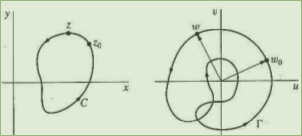
\includegraphics[scale=0.4]{ch7/image1.png}
	\captionof{figure}{Principe de l'argument}
\end{wrapfigure}
Ce principe est à la base de l'étude de la stabilité des boucles à régulations, comme 
nous aurons le plaisir de le voir en \textit{Automatique}.\\
Les hypothèses du théorème sont les suivantes : $f$ est analytique dans $D$, domaine
intérieur à $\mathcal{C}$ (admissible simple fermé orienté dans le sens positif) sauf 
aux pôles dans $D$. En outre, $f$ analytique et \textbf{non nulle} sur $\mathcal{C}$
(en rouge dans les slides).\\
Utilisions les notations  :\ \\
\begin{itemize}
	\item $\Gamma$ : l'image de $\mathcal{C}$ par transformation $w=f(z)$ qui ne passe pas
	      par l'origine.
	\item $\Delta_C\ arg\ f(z) = \phi_1-\phi_0$.
	\item $\frac{1}{2\pi}\Delta_C\ arg\ f(z) = T$ : nombre d'encerclements de l'origine par
	      $\Gamma$.
\end{itemize}\ \\
Avant d'énoncer le théorème, intéressons nous à la figure 7.1. Initialement, les points
$z$ et $z_0$ sont confondus, dont l'image est respectivement $w$ et $w_0$. Ensuite, 
ce point $z$ va parcourir le chemin $\mathcal{C}$ et $w$ va parcourir le chemin $\Gamma$. 
Quand $w$ revient en $w_0$, son argument (initialement $\phi_0$) s'est modifié ($\phi_1$). 
C'est donc un argument multiforme ou $\phi_0$ et $\phi_1$ sont multiplies l'un l'autre 
d'un multiple de $2\pi$ ; la division par $2\pi$ donne le nombre  d'encerclement\footnote{
	Ceci n'est pas vu en TP, mais revient souvent aux examens.}.\\

\theor{\textsc{Argument}\\
	\begin{equation}
		T = Z-P
	\end{equation}
	Le nombre d'encerclements de l'origine par $\Gamma$ est égal à la différence entre le
	nombre de pôles $P$ et de zéros $Z$ de $f(z)$ à l'intérieur de $\mathcal{C}$ (multiplicité
prise en compte).}


\begin{proof}\ \\
	Le but de la démonstration est d'évaluer $\int_C \frac{f'(z)}{f(z)}dz$ de deux façon différente.\\
	\textsc{Première méthode :} à partir de la définition de l'intégrale d'une fonction d'une
	variable complète.\\
	Soit $z=z(t), a\leq t\leq b$, l'équation paramétrique de $\mathcal{C}$. Compte-tenu de
	ceci, l'intégrale peut \^etre ré-écrite (substitution de la paramétrisation) :
	\begin{equation}
		\int_C\frac{f'(z)}{f(z)}dz = \int_a^b \frac{f'(z(t))z'(t)}{f(z(t))}dt
	\end{equation}
	Comme $\Gamma$ ne passe pas par l'origine, on peut utiliser les coordonnées polaires :
	$w = f(z(t)) = \rho(t)e^{i\phi(t)}, a\leq t\leq b$. Le numérateur donne :
	\begin{equation}
		f'(z(t))z'(t) = \frac{d}{dt}f(z(t)) = \frac{d}{dt}(\rho(t)e^{i\phi(t)}) = \rho'(t)e^{i
			\phi(t)} + i\rho(t)e^{i\phi(t)}\phi'(t)
	\end{equation}
	Cette expression permet de ré-écrire l'intégrale en deux parties qui existent bien comme 
	$\rho'(t)$ et $\phi'(t)$ sont continues par morceaux pour $a\leq t \leq b$ :
	\begin{equation}
		\int_C\frac{f'(z(t))}{f(z)} = \int_a^b \frac{\rho'(t)}{\rho(t)}dt + i\int_a^b \phi'(t)dt
		= \ln\rho(t)|_a^b + i\phi|_a^b
	\end{equation}
	Comme $\rho(a)=\rho(b)$, le premier terme s'annule pour finalement avoir :
	\begin{equation}
		\int_\mathcal{C} \frac{f'(z)}{f(z)}dz = i\Delta_C\ arg\ f(z)
	\end{equation}
	\textsc{Deuxième méthode} : théorème des résidus\\
	L'intégrante est analytique dans et sur $\mathcal{C}$ sauf aux pôles et zéros de $f$. Soit
	$z_0$, \textbf{zéro} d'ordre $m_0$ de $f$ :
	\begin{equation}
		f(z) = (z-z_0)^{m_0}g(z)
	\end{equation}
	avec $g(z)$ analytique en $z_0$ et $g(z_0)\neq0$. Nous savons que $f(z)$ peut s'écrire de 
	la sorte (cf. un peu plus haut). Regardons ce que donne $f'(z)$ :
	\begin{equation}
		f'(z_0) =  m_0(z-z_0)^{m_0-1}g(z) + (z-z_0)^{m_0}g'(z)
	\end{equation}
	Le rapport donne alors:
	\begin{equation}
		\frac{f'(z)}{f(z)} = \frac{m_0}{z-z_0}+\frac{g'(z)}{g(z)}
		\label{eq:DemoArg}
	\end{equation}
	Or $\frac{g'(z)}{g(z)}$ est analytique en $z_0$ et possède donc un développement en série
	de Taylor en puissance de $z-z_0$. Par \autoref{eq:DemoArg}, $\frac{g'(z)}{g(z)}$ possède 
	un p\^ole simple en $z_0$ avec un résidu $m_0$.\\
	De même manière, si $z_1$ est un \textbf{pôle} d'ordre $m_1$ de $f(z) ; f(z) = (z-z_1)^{-m_1}\phi(
	z)$ avec $\phi(z)$ analytique en $z_1$ et $\phi(z_1)\neq0$. L'intégrante possède un pôle 
	simple en $z_1$ avec $-m_1$ en résidu. Par le théorème des résidus :
	\begin{equation}
		\int_\mathcal{C} \frac{f'(z)}{f(z)}dz = 2\pi i(Z-P)
	\end{equation}
	En égalant les deux expressions obtenues par les deux méthodes :
	\begin{equation}
		i\Delta_\mathcal{C}\ arg\ f(z) = 2\pi i T = 2\pi i (Z-P)
	\end{equation}
\end{proof}
        
        
        
        
        
        
        
        
        